\begin{figure}
\begin{center}

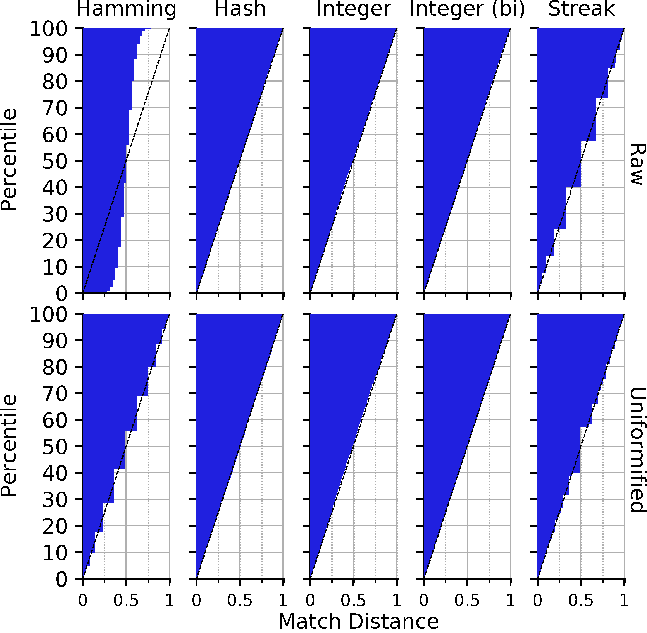
\includegraphics[width=\columnwidth]{img/uniformification/bitweight=0dot5+seed=1+title=low-score-distribution+_data_hathash_hash=75684cf1e73fb7f1+_script_fullcat_hash=c3113c80efb02374+ext=}
\caption{
Distance distributions of metrics before and after uniformification.
Each visualization arranges individually sampled observations (thin horizontal bars) vertically in descending order.
The $y$ axis can be interpreted as ranging form the 0th percentile of outcomes (bottom) to 100th percentile (top) with width of horizontal bars showing match distance at a certain percentile.
Dashed lines trace an ideal uniform distribution.
}
\label{fig:uniformification}

\end{center}
\end{figure}
